\documentclass[Arkitektur/System_main.tex]{subfiles}
\begin{document}
\subsubsection{Redigering af brugerprofil}
Når en bruger har lavet en brugerprofil og logget ind på profilen vil han eventuelt ændre personlige brugerinformation eller slette brugerprofilen. Arkitekturen for denne fremgangsmåde beskrives i dette afsnit, hvor der som det første vises sekevensdiagram, der beskriver samspillet mellem bruger, CarnGo applikationen og databasen (Figur \ref{fig:EditUserSD}). Herefter ses en applikations model, som inkluderer et klassediagram og et statemachine diagram.
\begin{figure}[H]
    \centering
    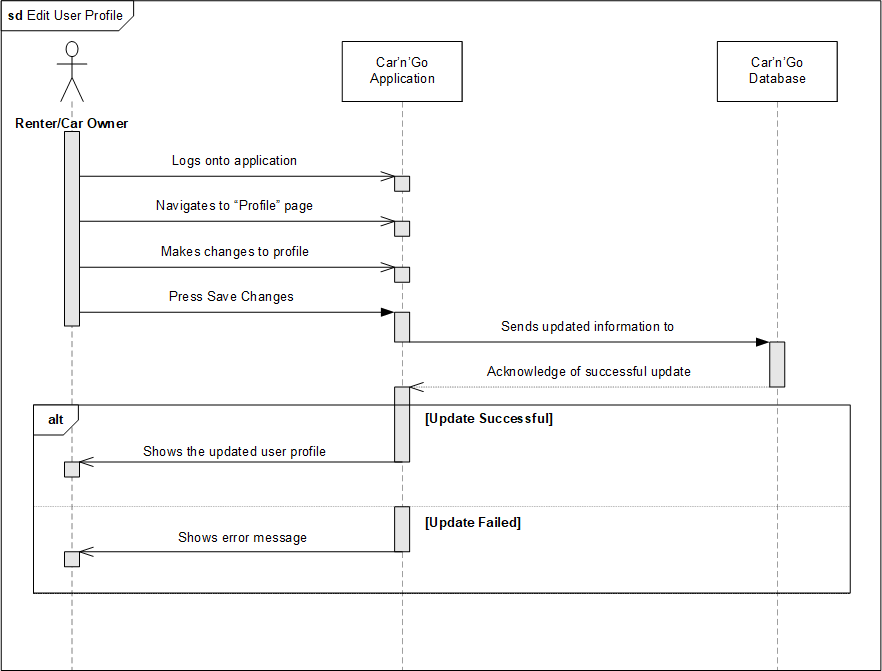
\includegraphics[width=1\textwidth]{Arkitektur/Softwarearkitektur/Edit_user_profile/graphics/SystemSD_ProfilerSD.png}
    \caption{Sekvensdiagram for redigering og fjernelse af en brugerprofil. }
    \label{fig:EditUserSD}
\end{figure}
Nedenfor ses applikationsmodellen, hvor der på figur \ref{fig:EditUserCD} vises et klassediagram og på figur \ref{fig:EditUserSTM} vises et statemachine diagram.
\begin{figure}[H]
    \centering
    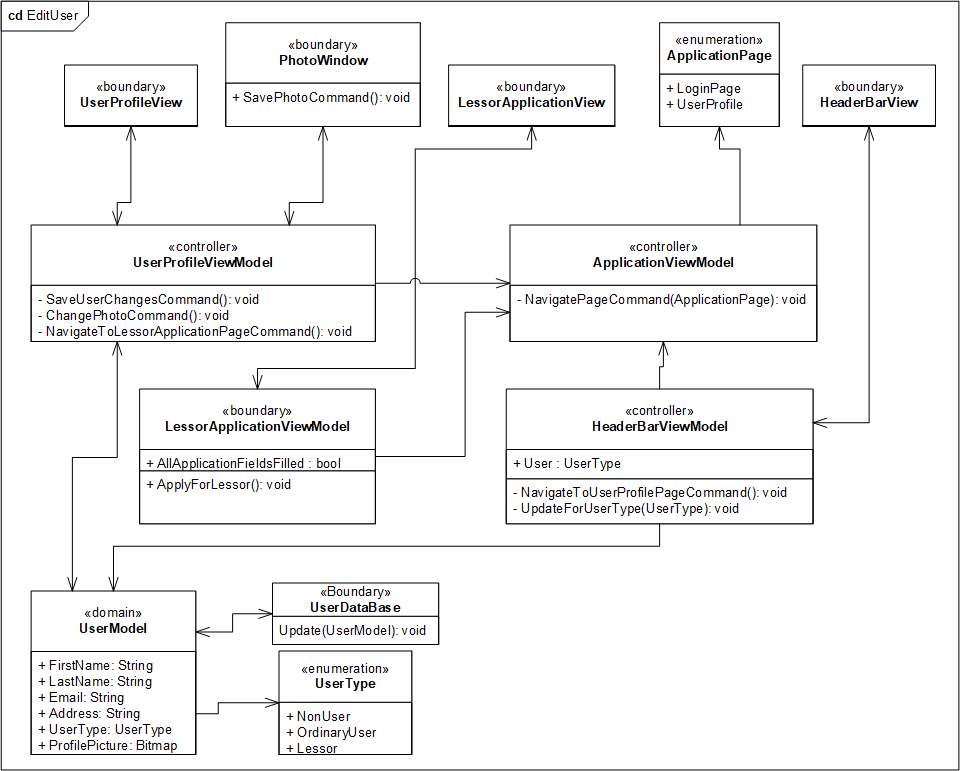
\includegraphics[width=1\textwidth]{Arkitektur/Softwarearkitektur/Edit_user_profile/graphics/EditUserCD.png}
    \caption{Klassediagram for redigering og fjernelse af en brugerprofil. }
    \label{fig:EditUserCD}
\end{figure}

\begin{figure}[H]
    \centering
    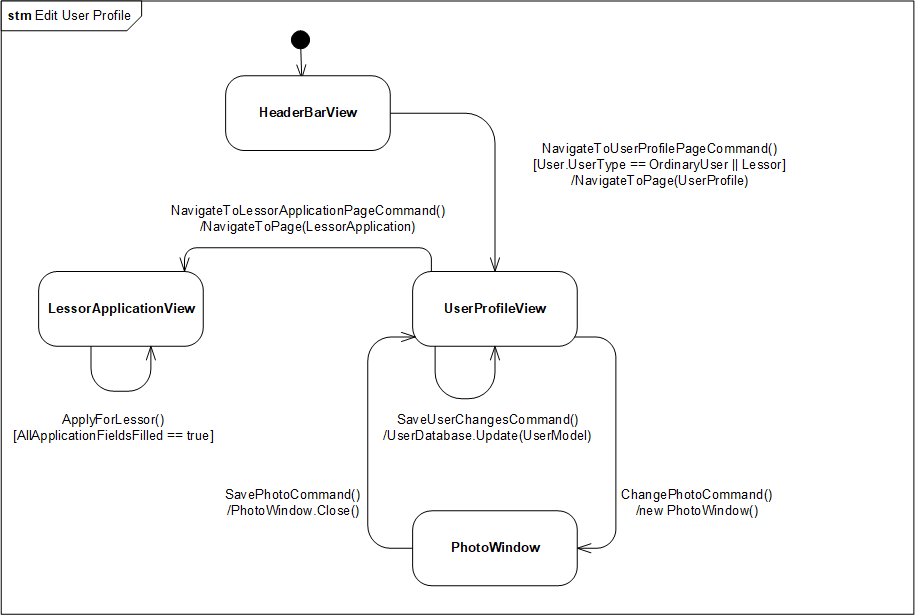
\includegraphics[width=1\textwidth]{Arkitektur/Softwarearkitektur/Edit_user_profile/graphics/EditUserSTM.png}
    \caption{Statemachine for redigering og fjernelse af en brugerprofil. }
    \label{fig:EditUserSTM}
\end{figure}




\end{document}